\documentclass[a4paper,11pt]{article}
\usepackage[T1]{fontenc}\usepackage[utf8]{inputenc}\usepackage{lmodern}\usepackage{microtype}
\usepackage[a4paper,margin=1in,headheight=15pt,headsep=14pt]{geometry}
\usepackage{amsmath,amssymb}\usepackage{graphicx}\usepackage{booktabs}
\usepackage[table,svgnames]{xcolor}\usepackage[most]{tcolorbox}\tcbuselibrary{skins,breakable}
\usepackage{tikz}\usepackage{pifont}\usepackage{bbding}\usepackage{enumitem}
\setlist{leftmargin=1.5em,topsep=4pt,itemsep=3pt}\usepackage{parskip}
\usepackage{fancyhdr}\usepackage{titlesec}\usepackage[hidelinks]{hyperref}\usepackage{xurl}
\hypersetup{breaklinks=true}
\definecolor{navy}{HTML}{21355E}\definecolor{navyrule}{HTML}{21355E}
\definecolor{inktext}{HTML}{1A202C}\definecolor{mutedtext}{HTML}{6B7280}
\definecolor{intuFrame}{HTML}{2C5AA0}\definecolor{intuFill}{HTML}{F4F7FC}
\definecolor{everyFrame}{HTML}{8A5A1E}\definecolor{everyFill}{HTML}{FBF1E3}
\definecolor{workFrame}{HTML}{2E7D52}\definecolor{workFill}{HTML}{F1F8F3}
\definecolor{watchFrame}{HTML}{B23A48}\definecolor{watchFill}{HTML}{FBF1F2}
\definecolor{keyFrame}{HTML}{6A4C93}\definecolor{keyFill}{HTML}{F4F0F9}
\color{inktext}\hypersetup{linkcolor=navy,urlcolor=navy,citecolor=navy}
\tcbset{housecallout/.style 2 args={enhanced,breakable,colback=#2,colframe=#1,boxrule=0.6pt,arc=2.4pt,outer arc=2.4pt,left=10pt,right=10pt,top=9pt,bottom=9pt,before skip=11pt,after skip=11pt,fontupper=\normalsize,coltitle=white,fonttitle=\bfseries\sffamily\small,attach boxed title to top left={xshift=6mm,yshift=-3mm},boxed title style={colback=#1,colframe=#1,rounded corners,arc=3pt,boxrule=0pt,left=6pt,right=6pt,top=2pt,bottom=2pt}}}
\newtcolorbox{intuition}{housecallout={intuFrame}{intuFill},title={\raisebox{-0.05ex}{\Pointinghand}\,\ The intuition}}
\newtcolorbox{everyday}{housecallout={everyFrame}{everyFill},title={\raisebox{-0.05ex}{$\bigstar$}\,\ Everyday picture}}
\newtcolorbox{worked}[1]{housecallout={workFrame}{workFill},title={\raisebox{-0.05ex}{\Pencil}\,\ Worked example: #1}}
\newtcolorbox{watchout}{housecallout={watchFrame}{watchFill},title={\raisebox{-0.05ex}{\ding{55}}\,\ Watch out}}
\newtcolorbox{keytake}{housecallout={keyFrame}{keyFill},title={\raisebox{-0.05ex}{\ding{51}}\,\ Key takeaway}}
\newcommand{\CourseShort}{SEML Companion}\newcommand{\SessionNo}{2}\newcommand{\LectureTitle}{ML in Production}
\pagestyle{fancy}\fancyhf{}
\fancyhead[L]{\footnotesize\color{mutedtext}\textsf{\CourseShort}}
\fancyhead[R]{\footnotesize\color{mutedtext}\textsf{Session \SessionNo\ \textperiodcentered\ \LectureTitle}}
\fancyfoot[C]{\footnotesize\color{mutedtext}\thepage}
\renewcommand{\headrulewidth}{0.4pt}\renewcommand{\footrulewidth}{0pt}
\renewcommand{\headrule}{\hbox to\headwidth{\color{navyrule!55}\leaders\hrule height \headrulewidth\hfill}}
\titleformat{\section}{\sffamily\Large\bfseries\color{navy}}{\thesection}{0.8em}{}[{\vspace{2pt}\color{navy!70}\titlerule[0.8pt]}]
\titleformat{\subsection}{\sffamily\large\bfseries\color{navy!92}}{\thesubsection}{0.7em}{}
\titlespacing*{\section}{0pt}{16pt}{8pt}\titlespacing*{\subsection}{0pt}{12pt}{4pt}
\newcommand{\titlebanner}[4]{\begin{tcolorbox}[enhanced,breakable=false,colback=navy,colframe=navy,boxrule=0pt,arc=3pt,outer arc=3pt,left=16pt,right=16pt,top=16pt,bottom=16pt,before skip=2pt,after skip=14pt,width=\linewidth]{\sffamily\footnotesize\bfseries\color{white!85}\MakeUppercase{#1}}\par\vspace{6pt}{\sffamily\bfseries\fontsize{30}{34}\selectfont\color{white}#2\par}\vspace{5pt}{\sffamily\large\color{white!88}#3\par}\vspace{9pt}{\color{white!55}\rule{\linewidth}{0.4pt}}\par\vspace{6pt}{\sffamily\footnotesize\color{white!82}#4\par}\end{tcolorbox}}
\newcommand{\vocab}[1]{\textbf{\color{navy}#1}}
\begin{document}
\thispagestyle{fancy}
\titlebanner{AIMLCZG546 · Session 2 · Companion Reader}{Machine Learning in Production}{From Research Prototype to Production System: Scope, Challenges, and Architecture}{Session 2 · Read alongside the lecture slides · Every concept and case study explained in full}

\noindent\textbf{How to use this companion.} Five colour-coded boxes appear throughout. \textcolor{intuFrame}{\textbf{Blue}} = core intuition. \textcolor{everyFrame}{\textbf{Amber}} = everyday analogy. \textcolor{workFrame}{\textbf{Green}} = worked scenario. \textcolor{watchFrame}{\textbf{Red}} = pitfall. \textcolor{keyFrame}{\textbf{Purple}} = the one line to remember.

%==============================================================
\section{The Production Gap: Sidney's Startup}
%==============================================================

A common story in ML: a talented researcher builds an impressive model in a notebook. Accuracy is high on the test set. Everyone is excited. Then they try to deploy it. That is when the real work begins.

\begin{everyday}
A chef perfects a recipe at home for six people. Then a restaurant chain wants to serve it to 10{,}000 people per day across 50 cities. The recipe itself is only a tiny part of the problem. The real challenges are: sourcing consistent ingredients, training kitchen staff, maintaining quality control, handling customer complaints, and managing costs.
\end{everyday}

\vocab{Sidney} builds a speech recognition model for customer calls. In the lab, accuracy is 94\,\%. In production, he encounters:

\begin{itemize}
  \item \textbf{Noisy real-world data} --- call centre audio has background noise, accents, and technical jargon not in the training set.
  \item \textbf{Latency constraints} --- the model must respond in under 500\,ms; the research model takes 3\,seconds.
  \item \textbf{Cloud cost explosion} --- running the model 24/7 at scale costs 40$\times$ the research estimate.
  \item \textbf{Pipeline fragility} --- the data preprocessing script breaks when the call centre upgrades its recording format.
  \item \textbf{Team gaps} --- ML researchers and software engineers don't share vocabulary or tools.
  \item \textbf{Monitoring failures} --- accuracy degrades after six months (customers' language changed) but nobody notices for three weeks.
  \item \textbf{Fairness gaps} --- the model performs 15\,\% worse on non-native English speakers.
\end{itemize}

\begin{keytake}
Moving from research prototype to production system requires as much engineering effort as building the model itself --- often more.
\end{keytake}

%==============================================================
\section{ML Model vs ML System}
%==============================================================

There are two very different ways to think about an ML project.

\subsection{Model-Centric View}

A \vocab{model-centric} team asks: ``How do we make the model more accurate?'' They tune hyperparameters, try new architectures, and collect more labelled data. Improvement stops when the model tops out.

\subsection{System-Centric View}

A \vocab{system-centric} team asks: ``How do we make the entire end-to-end system better for users?'' The model is one component of a larger system. Improvements can come from better data pipelines, faster infrastructure, better monitoring, or better UX --- not just the model.

\begin{intuition}
An ML model is like an engine in a car. A better engine helps, but the car's usefulness also depends on the chassis, the steering, the tyres, the fuel system, and the driver interface. Optimising only the engine while ignoring everything else is model-centric thinking.
\end{intuition}

\subsection{The Iceberg of Hidden Technical Debt}

Sculley et al. (2015) --- a landmark paper from Google --- showed that the actual ML code in a production system is a tiny fraction of the total codebase. The rest is the infrastructure:

\begin{center}
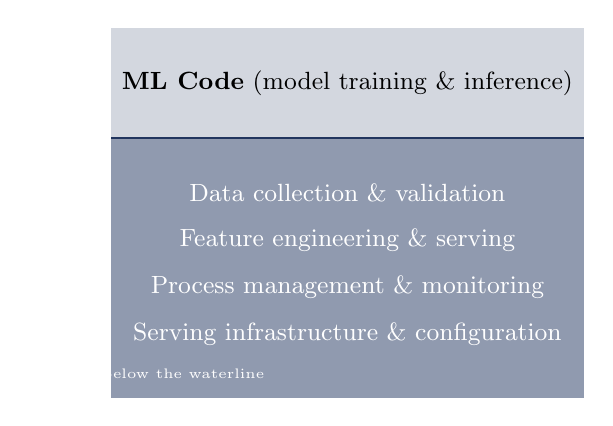
\begin{tikzpicture}[font=\small]
  \fill[navy!20] (-3,-0.2) -- (3,-0.2) -- (3,1.2) -- (-3,1.2) -- cycle;
  \fill[navy!50] (-3,-3.5) -- (3,-3.5) -- (3,-0.2) -- (-3,-0.2) -- cycle;
  \draw[thick,navy] (-3,-0.2) -- (3,-0.2);
  \node[align=center] at (0,0.5) {\textbf{ML Code} (model training \& inference)};
  \node[align=center,white] at (0,-0.9) {Data collection \& validation};
  \node[align=center,white] at (0,-1.5) {Feature engineering \& serving};
  \node[align=center,white] at (0,-2.1) {Process management \& monitoring};
  \node[align=center,white] at (0,-2.7) {Serving infrastructure \& configuration};
  \node[align=left,white,font=\tiny] at (-2.5,-3.2) {Hidden below the waterline};
\end{tikzpicture}
\end{center}

\begin{watchout}
Optimising the ML model while neglecting the infrastructure is like polishing the engine while the fuel tank leaks. The fuel tank will kill the car first.
\end{watchout}

\begin{worked}{Model-centric vs system-centric fraud detection}
A bank's fraud detection model has 88\,\% precision (12\,\% false positives --- legitimate transactions blocked). \\[4pt]
\textbf{Model-centric fix:} Collect more labelled fraud examples. Retrain with XGBoost. New precision: 90\,\%. Cost: 3 weeks. \\[4pt]
\textbf{System-centric fix:} Analyse why false positives occur. Discovery: the feature pipeline is using yesterday's exchange rates for international transactions. Fix the pipeline. New precision: 93\,\%, with no model change at all. Cost: 2 days. \\[4pt]
The system-centric approach found a bigger gain faster by looking beyond the model.
\end{worked}

%==============================================================
\section{ML and Non-ML Components in a System}
%==============================================================

Real production systems mix ML and traditional software. The ML component may be central (\vocab{core}) or supporting (\vocab{auxiliary}).

\begin{center}
\resizebox{\linewidth}{!}{%
\begin{tabular}{lll}
\toprule
\textbf{System} & \textbf{ML role} & \textbf{Non-ML components} \\
\midrule
Speech transcription service & Core (the product IS the ML output) & Audio codec, API gateway, billing \\
Tax software audit risk & Auxiliary (flags for human review) & Form parsing, rule engine, UI, tax database \\
E-commerce recommendation & Core (drives revenue directly) & Product catalogue, cart, payment, logistics \\
\bottomrule
\end{tabular}}
\end{center}

\noindent\textbf{Where this shows up in ML/AI.} Systems thinking means you must design every non-ML component around the ML component's failure modes. When the fraud model makes a mistake, who sees it, what happens next, and how do you recover? These are software engineering questions, not ML questions.

%==============================================================
\section{AI Paradigms: Predictive, Generative, and Agentic}
%==============================================================

Modern AI systems fall into three paradigms, each with different capabilities and engineering requirements.

\subsection{Predictive AI}

\vocab{Predictive AI} uses past data to predict future outcomes. The model is trained on historical data and answers a specific question (``Will this customer churn?'', ``Is this email spam?''). Output is a number, a label, or a probability.

\subsection{Generative AI}

\vocab{Generative AI} creates new content based on patterns learned from data. A foundation model is given a natural-language instruction and produces a digital artefact: text, code, an image, a video.

\begin{intuition}
Predictive AI is like a detective who studies evidence and says ``the suspect is probably the butler.'' Generative AI is like a novelist who reads a thousand mystery novels and then writes a new one.
\end{intuition}

\subsection{Agentic AI}

\vocab{Agentic AI} acts autonomously to achieve a goal. It combines reasoning (planning multi-step actions), tools (calling APIs, searching the web, running code), and feedback loops (evaluating its own output and correcting errors).

\[
\text{Agentic AI} = \text{Generative AI} + \text{Reasoning} + \text{Tools} + \text{Feedback Loops}
\]

\begin{everyday}
Predictive AI is a weather forecast app: you ask, it answers. Generative AI is a ghostwriter who drafts the email you asked for. Agentic AI is a personal assistant who reads your brief, books the flight, writes the agenda, sends the meeting invite, and then revises the agenda when you tell them the venue changed.
\end{everyday}

\begin{keytake}
Agentic AI systems are not just smarter chatbots --- they are autonomous software agents that can take sequences of real-world actions. This changes the SE challenges significantly (coordination, safety, rollback).
\end{keytake}

%==============================================================
\section{Cloud-Native ML Systems}
%==============================================================

\vocab{Cloud-native} software is designed from the start to run on cloud infrastructure using containers, microservices, and automated deployment. The Cloud Native Computing Foundation (CNCF) defines it as: technologies that use containers, service meshes, microservices, immutable infrastructure, and declarative APIs.

For ML systems, cloud-native means:
\begin{itemize}
  \item Models run in containers (reproducible, isolated environments).
  \item Training and serving scale independently (more GPUs for training; more API servers for serving).
  \item Infrastructure is defined as code (Terraform, Kubernetes YAML) so it is versioned and auditable.
  \item ML workloads are the dominant and fastest-growing type of cloud compute today.
\end{itemize}

%==============================================================
\section{Case Study: Apollo Autonomous Driving (Baidu)}
%==============================================================

Baidu's Apollo platform is one of the most complex ML systems ever deployed in a safety-critical context. It illustrates what ``ML system'' means at industrial scale.

Apollo uses \textbf{28 ML models} across three functional areas:
\begin{itemize}
  \item \textbf{Perception} --- cameras and LiDAR sensors feed models that detect lanes, vehicles, pedestrians, traffic signs, and road boundaries.
  \item \textbf{Detection \& Classification} --- models classify objects and predict their type (car, cyclist, pedestrian).
  \item \textbf{Trajectory Prediction} --- models forecast where detected objects will be in the next 3--5 seconds.
\end{itemize}

\begin{worked}{Model interaction in Apollo}
The pipeline for a single frame of camera data: \\
\textbf{Step 1:} Raw camera image (1920$\times$1080, 30 fps) is received. \\
\textbf{Step 2:} Object Detection model (YOLOv5 variant) runs. Output: 14 bounding boxes (cars, pedestrians, cyclists). \\
\textbf{Step 3:} Each bounding box is fed to the Classification model. Output: ``Car (0.97), Pedestrian (0.91), Truck (0.83)...'' \\
\textbf{Step 4:} Classification outputs + LiDAR point cloud are fused by the Multi-Sensor Fusion model. Output: 3D positions of all objects. \\
\textbf{Step 5:} Trajectory Prediction model takes 3D positions + velocity history. Output: predicted paths for next 4 seconds. \\
\textbf{Step 6:} Motion Planning (rule-based + ML) uses predicted paths to compute a safe driving trajectory. \\
\textbf{Step 7:} Control system executes the trajectory (steering, throttle, brake). \\[4pt]
If Step 2 produces a false negative (misses a pedestrian), every downstream step receives wrong input. This cascading failure risk is the core SE challenge of multi-model systems.
\end{worked}

\noindent\textbf{SE4ML challenges in Apollo:} high system complexity (28 interacting models), very low test coverage (hard to write unit tests for probabilistic models), model maintenance (each of 28 models must be versioned and retrained separately), and safety requirements (a wrong prediction may kill someone).

%==============================================================
\section{Case Study: Microsoft's 9-Stage ML Workflow}
%==============================================================

Microsoft studied how ML is embedded in Agile engineering teams and found a consistent 9-stage workflow.

\begin{center}
\resizebox{\linewidth}{!}{%
\begin{tabular}{rll}
\toprule
\textbf{Stage} & \textbf{Name} & \textbf{Key question} \\
\midrule
1 & Model Requirements & What problem are we solving? What does success look like? \\
2 & Data Collection & Where does the data come from? Is it available? \\
3 & Data Cleaning & Is the data accurate, complete, and consistent? \\
4 & Data Labelling & Do we have ground truth? Who labels it? \\
5 & Feature Engineering & What signals will help the model? \\
6 & Model Training & What algorithm? What hyperparameters? \\
7 & Model Evaluation & Does it meet the performance requirements? \\
8 & Deployment & How is the model served? What latency / throughput? \\
9 & Monitoring & Is the model still performing well in production? \\
\bottomrule
\end{tabular}}
\end{center}

Key findings from Microsoft's research:
\begin{itemize}
  \item \textbf{Data is the central engineering activity.} More time is spent on stages 2--5 than on 6--7.
  \item \textbf{Experimentation-driven development.} Teams run dozens of experiments before choosing a model.
  \item \textbf{Cross-functional teams are essential.} ML engineers, data engineers, domain experts, and product managers must collaborate from stage 1.
  \item \textbf{Versioning is not optional.} Both models and datasets must be versioned to ensure reproducibility.
\end{itemize}

\begin{keytake}
In the Microsoft workflow, the model training stage (Stage 6) is preceded by four data-intensive stages. ``Data first, model second'' is the industrial reality.
\end{keytake}

\end{document}
